
\section{LI-rezoluce}\label{section:predicate-LI-resolution}

V této sekci připomeneme pojmy \alert{lineárního a linear-input důkazu}, \alert{LI-rezoluci} a její úplnost pro Hornovské formule. Definice i znění vět jsou stejné jako ve výrokové logice (jediným rozdílem je, že v důkazech můžeme používat \alert{varianty} klauzulí z $S$), důkaz lze provést převedením na výrokovou logiku opět pomocí Herbrandovy věty a Lifting lemmatu.

\begin{definition}[Lineární a LI důkaz]
    \alert{Lineární důkaz} (rezolucí) klauzule $C$ z formule $S$ je konečná posloupnost
    $$
    \begin{bmatrix}
        C_0 \\
        B_0
    \end{bmatrix},
    \begin{bmatrix}
        C_1 \\
        B_1
    \end{bmatrix},\dots,
    \begin{bmatrix}
        C_n \\
        B_n
    \end{bmatrix},
    C_{n+1}
    $$
    kde $C_i$ říkáme \alert{centrální} klauzule, $C_0$ je \alert{počáteční}, $C_{n+1}=C$ je \alert{koncová}, $B_i$ jsou \alert{boční} klauzule, a platí:
    \begin{itemize}
        \item $C_0$ je varianta klauzule z $S$, pro $i\leq n$ je $C_{i+1}$ rezolventou $C_i$ a $B_i$,
        \item $B_0$ je varianta klauzule z $S$, pro $i\leq n$ je $B_i$ varianta klauzule z $S$ nebo $B_i=C_j$ pro nějaké $j<i$. 
    \end{itemize}
    \alert{Lineární zamítnutí} $S$ je lineární důkaz $\square$ z $S$.
    
    \alert{LI-důkaz} je lineární důkaz, ve kterém je každá boční klauzule $B_i$ variantou klauzule z $S$. Pokud existuje LI-důkaz, říkáme, že je $C$ \alert{LI-dokazatelná} z $S$, a píšeme $S\proves_{LI}C$. Pokud $S\proves_{LI}\square$, je $S$ \alert{LI-zamítnutelná}.
\end{definition}

V Poznámce \ref{remark:linear-resolution} jsme poznamenali, že `lineární' rezoluce (založená na lineárních důkazech) je úplná. Důkaz byl ponechán jako cvičení. Stejné tvrzení platí i v predikátové rezoluci:

\begin{theorem}[O úplnosti lineární rezoluce]
Klauzule $C$ má lineární důkaz z CNF formule $S$, právě když má rezoluční důkaz z $S$ (tj. $S\proves_R C$).
\end{theorem}
\begin{proof}
Z lineárního důkazu snadno vyrobíme rezoluční strom. Opačná implikace plyne z Poznámky \ref{remark:linear-resolution} a z Lifting lemmatu (jehož použití zachovává linearitu rezolučního důkazu).
\end{proof}

\subsection{Úplnost LI-rezoluce pro Hornovy formule}

Připomeňme terminologii týkající se hornovskosti a programů: \alert{Hornova klauzule} je klauzule obsahující nejvýše jeden pozitivní literál. \alert{Hornova formule} je (konečná, nebo i nekonečná) množina Hornových klauzulí.
\alert{Fakt} je pozitivní jednotková (Hornova) klauzule, \alert{pravidlo} je (Hornova) klauzule s právě jedním pozitivním a alespoň jedním negativním literálem, a \alert{cíl} je neprázdná (Hornova) klauzule bez pozitivního literálu. Pravidlům a faktům říkáme \alert{programové klauzule}.

Stejně jako ve výrokové logice, LI-rezoluce je úplná pro Hornovské formule:

\begin{theorem}[O úplnosti LI-rezoluce pro Hornovy formule]\label{theorem:completeness-of-li-resolution-for-horn-predicate}
Je-li Hornova formule $T$ splnitelná, a $T\cup\{G\}$ je nesplnitelná pro cíl $G$, potom $T\cup\{G\}\proves_{LI}\square$, a to LI-zamítnutím, které začíná cílem $G$.   
\end{theorem}
\begin{proof}
    Plyne z analogické věty ve výrokové logice, z Herbrandovy věty, a z Lifting lemmatu
\end{proof}


\subsection{(draft) Rezoluce v Prologu}\todo

% from slides:
\subsubsection*{Program v Prologu}
    \mdef{Program} (v Prologu) je Hornova formule obsahující pouze \myblue{programové}
    \smallskip
    
    \myblue{klauzule}, tj. \myblue{fakta} nebo \myblue{pravidla}.
    \bigskip
    
    \centerline{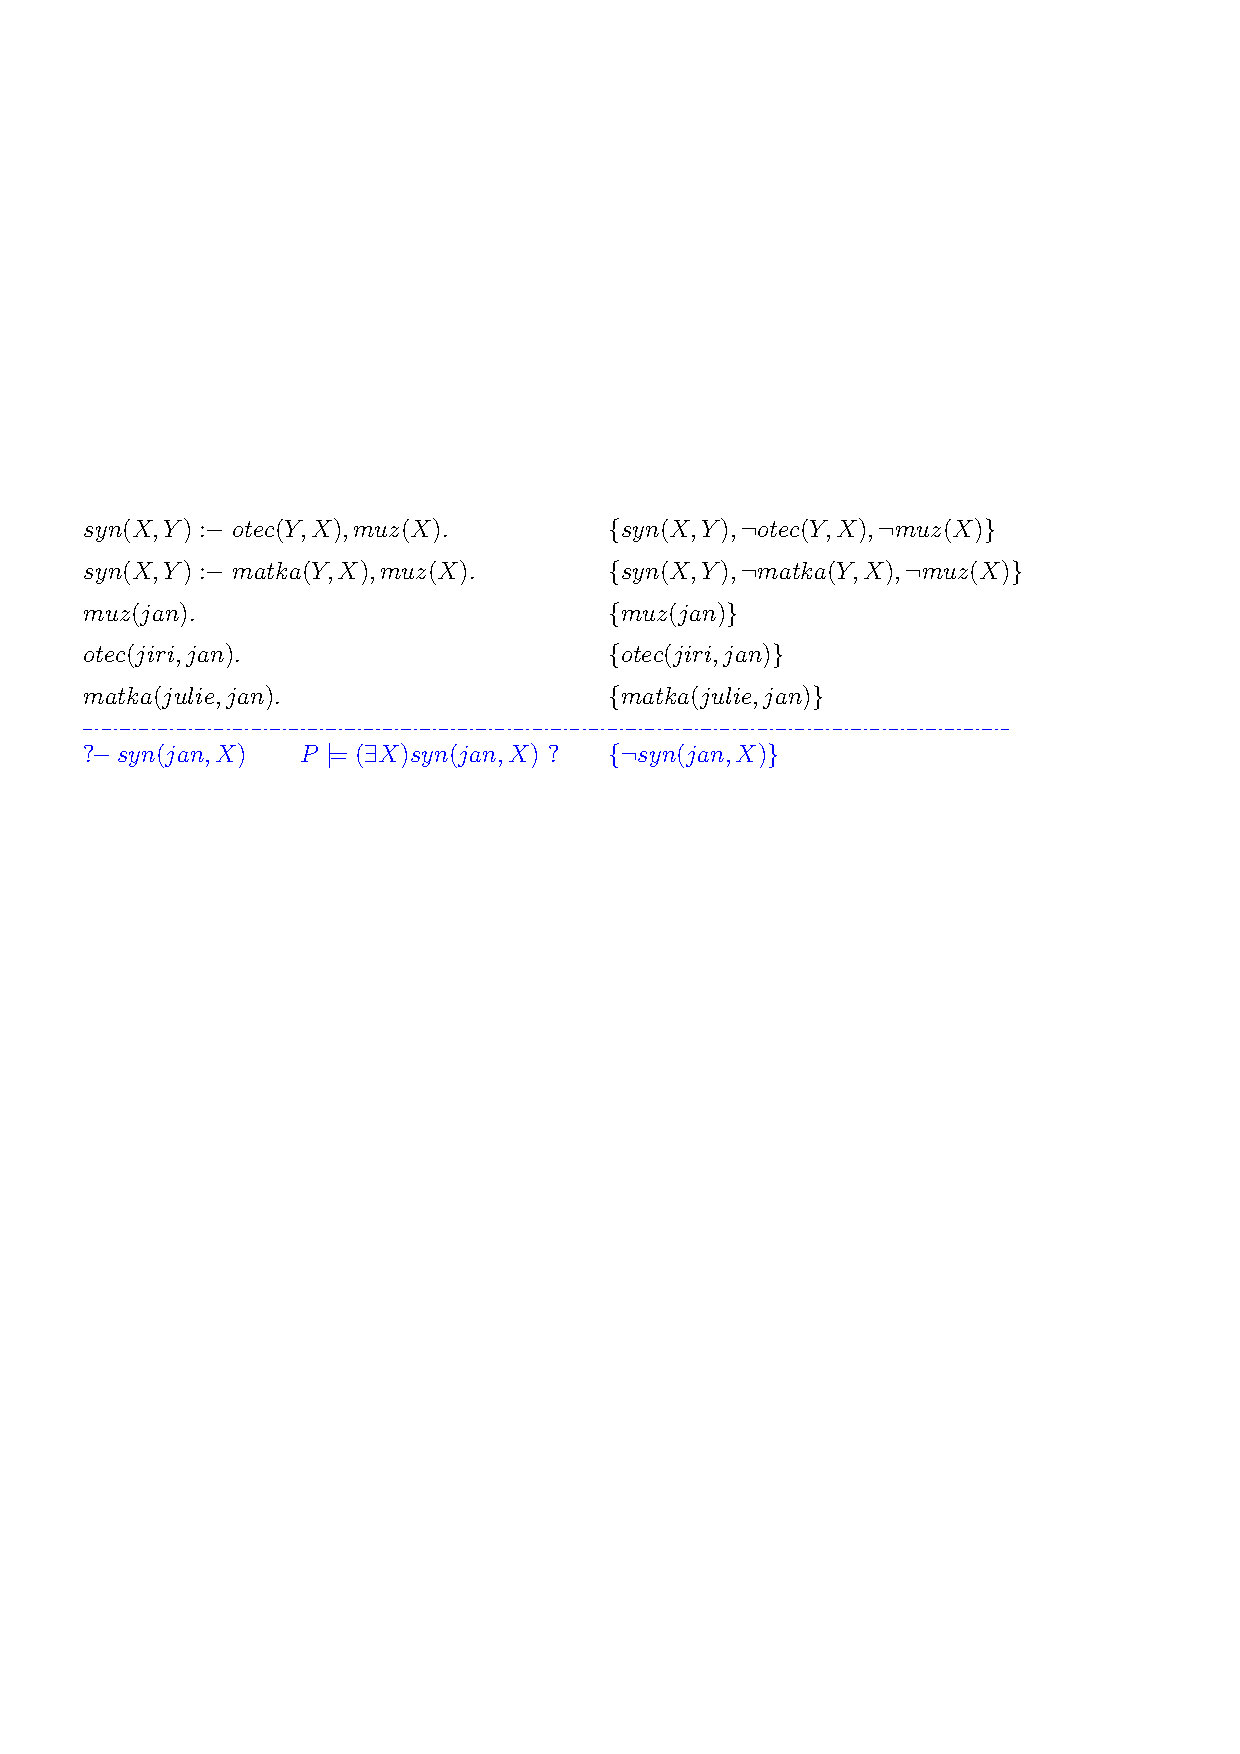
\includegraphics[scale=0.7]{files/rezolucePLprogram}}
    \bigskip
    
    {\it Zajímá nás, zda daný \myblue{existenční dotaz} vyplývá z daného programu.}%, navíc to chceme doložit \myblue{výstupní substitucí}.
    \medskip
    
    {\bf \myblue{Důsledek}}\ \ {\it Pro program $P$ a cíl $G=\{\neg A_1, \dots, \neg A_n\}$ v proměnných $X_1,\dots,X_m$
    
    \vspace{-0mm}
    \begin{enumerate}
    \item[$(1)$] $P \models (\exists X_1)\dots(\exists X_m)(A_1\mand \dots \mand A_n)$, právě když
    \smallskip
    
    \item[$(2)$] $\square$ lze odvodit LI-rezolucí z $P\cup\{G\}$ začínající (variantou) cíle $G$.
    \end{enumerate}}
    
    
    %%%%%%%%%%%%%%%%%%%%%%%%%%%%%%%%%%%%%%%%%%%%%%%%%%%%%%5
    
    \subsubsection*{LI-rezoluce nad programem}
    {\it Je-li odpověď na dotaz kladná, chceme navíc znát výstupní substituci.}
    \medskip
    
    \mdef{Výstupní substituce} $\sigma$ LI-rezoluce $\square$ z $P\cup\{G\}$ začínající $G=\{\neg A_1,\dots,\neg A_n\}$
    \smallskip
    
    je složení \myblue{mgu} v jednotlivých krocích (jen na proměnné v $G$). Platí,
    \vspace{-2mm}
    \mygreen{$$P \models (A_1 \mand \dots \mand A_n)\sigma.$$}
    
    \vspace{-2mm}
    
    \centerline{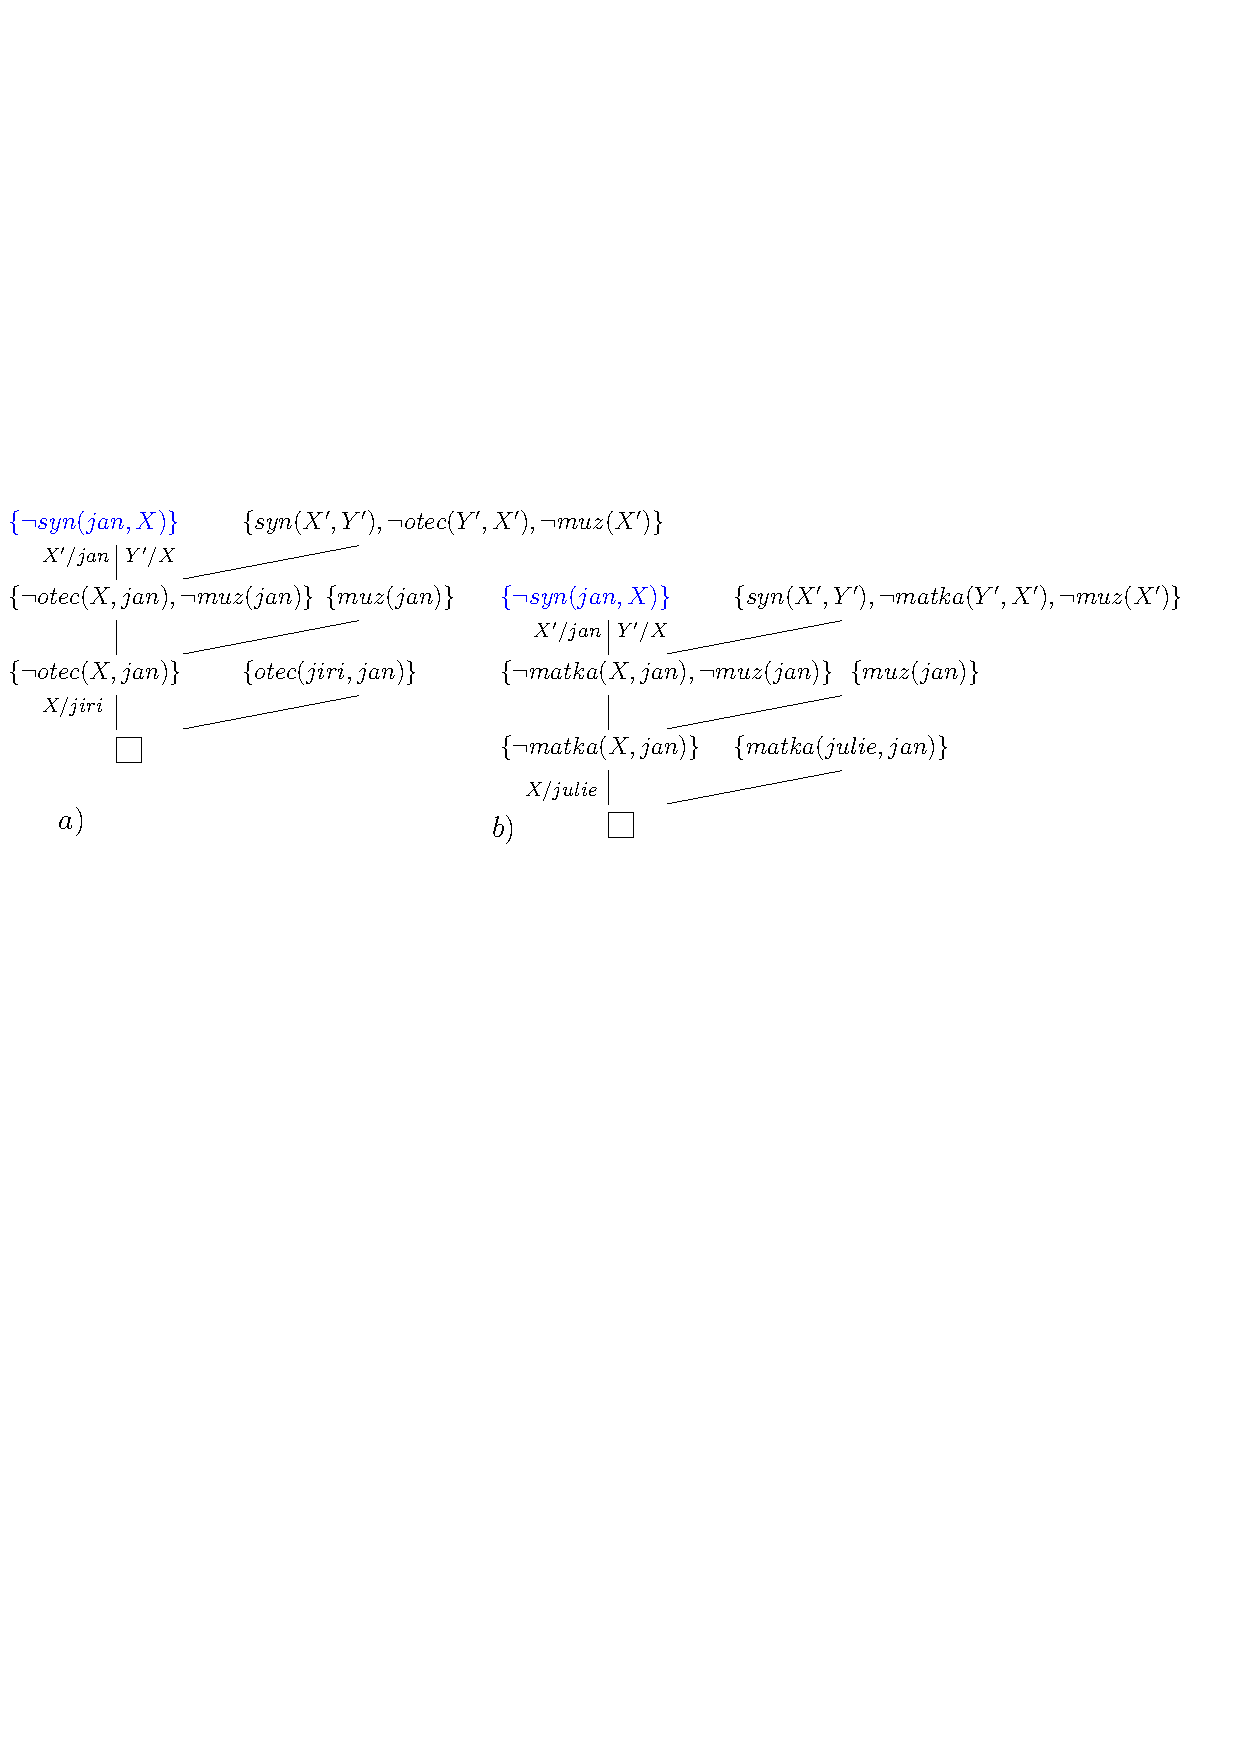
\includegraphics[scale=0.63]{files/rezolucePLprogramLI}}
    \bigskip
    
    Výstupní substituce $a)$ $X=jiri$,\ \ $b)$ $X=julie$.
    
    
% :from slides
